\chapter{The Polarization of Light}

\chapterprecis{Optics Practicum 1}

\makeoddhead{myheadings}{\emph{The Polarization of Light}}{}{\thepage}
\makeevenhead{myheadings}{\thepage}{}{\emph{Practicum}}

\section*{Introduction}

In Planck, Einstein, and Bohr, we’ve seen that light, previously thought to be wave-like, exhibits behavior characteristic of discrete, particle-like quanta. In de Broglie, we’ve seen that at least one body previously thought to be particle-like, the electron, exhibits wave-like behaviors, both when confined to the atom and when moving freely. In this portion of the semester, we will return to the study of photons, but now with the further complications introduced by Schr\"odinger’s and Heisenberg’s extension of the “matter wave” theory and attempts to set mechanics on a new footing. Paul Dirac’s \emph{Principles of Quantum Mechanics} continues this work, and while part of what makes the book so important is its new theory of the electron, we will read only the Introduction, where Dirac
elaborates some of the key features of his account not with reference to electrons, but in terms of the behavior of photons.\footnote{Though, as Dirac notes, ``The association of particles with waves discussed above is not
	restricted to the case of light, but is, according to modern theory, of universal applicability'' (Introduction, 
	sec.\ 3).}

One element of that behavior that will be important for Dirac’s account---as well as for much of the substantial 
experimental work we have left to do this term---is polarization. In 1690, Christian Huygens discovered 
the key phenomenon while investigating the Iceland spar (or clear calcite) crystal. Light passing through the
crystal was refracted into two differently directed rays, one obeying the usual laws of refraction, the other apparently not. 
Further, when Huygens placed one crystal atop another in the same orientation, he found that the two rays were not split a second time. In this orientation, the extrordinary ray was again irregularly refracted, and the ordinary ray regularly refracted, but when one of these crystals was then rotated in the plane of their contact by 90 degrees, the converse occurred. Huygens hypothesized that the two rays were composed of two distinct species of light, filtered, as it were, by the crystal: ``One would say that [the regular ray] in passing through the upper piece [of crystal] has lost something which is necessary to move the matter which serves for the irregular refraction; and that likewise [the irregular ray] has lost that which was necessary to move the matter which serves for regular refraction.''\footnote{Christian Huygens, \emph{Trait\'e de la lumi\`ere} (Paris, 1690), 90.} (Examination of the refraction in the crystal is proposed in section (J) below.)

Little to no progress in understanding was made in the 18th century, but a few related phenomena were uncovered in the 19th, two of them important and relevant to us. First, around 1810, \'Etienne-Louis Malus published the results of his research into polarization, showing that light reflected from an otherwise transparent surface and entering a suitably oriented Iceland spar crystal was \emph{not} split into two rays, and further, that when direct light was made to enter the crystal and split, and then the two rays exiting the crystal were projected onto water, only one was reflected. In investigating the effect of other orientations of the crystal on the quantity of light transmitted, Malus formulated a law that quantitatively expresses this relation, which we will employ extensively and discuss presently. Indeed, Malus's identification of what appeared to him as an orientation of light itself is what led him to dub the phenomenon ``polarization.'' Second, Faraday dis\-co\-ve\-red that the axis of polarization of light could be sensibly rotated by a sufficiently pow\-er\-ful mag\-net\-ic field, especially when the light was made to pass through a dense medium such as water.\footnote{See Faraday, \emph{Experimental Researches in Electricity,} Nineteenth Series, \emph{Phil. Trans. R. Soc. Lond.} \textbf{122} (1846), 1--20, and Maxwell, ``A Dynamical Theory of the Electric Field,'' article 8.} A theory that could plausibly account for polarization (among many other phe\-nom\-e\-na) arrived with Maxwell. Light, he asserted, is electromagnetic radiation, an electric and a magnetic wave---perpendicular to and in phase with each other---propagating through the luminiferous ether. On that account, the phenomena of polarization are easy to understand. The electric and magnetic components of the wave can, so long as they remain mutually perpendicular, point in any direction in the plane perpendicular to the wave’s direction of propagation, as the radius of a circle can connect the center with any point on its circumference. Polarization, then, would be made possible by the two-dimensional freedom of direction of oscillation characteristic of a transverse wave, in this case, that of light's electric and magnetic components. On this view, what Huygens saw in the Iceland spar could be explained by hypothesizing that the crystal divides unpolarized light into differently directed portions.\footnote{Maxwell discusses the electromagnetic theory of polarization and relates the polarizing effect of birefringent materials to the differing dielectric constant in different directions in the crystals in \emph{A Treatise on Electricity and Magnetism} (Oxford, 1873), articles 791--797. He discusses Faraday's demonstration and the effect of magnetism on polarization in articles 806--831.}

Soon, when we turn to Dirac, we will have to grapple with the quantum character of light once again, but for now, we
will familiarize ourselves further with the phenomena of polarization in terms in which it is adequately accounted 
for---and perhaps most naturally expressed---namely, those of classical electromagnetic theory. A bit of terminology: as the light wave progresses, if the axis of oscillation of the electric field remains fixed, the light is said to be \emph{linearly polarized}; if instead it rotates, the light is said to be \emph{elliptically polarized}; in the special case of elliptical polarization where the electric vector rotates \emph{and} maintains the same amplitude through\-out its rotation, the light is \emph{circularly polarized}. We will explore mostly linear polarization, though knowledge of the other forms is necessary for understanding some of the more com\-pli\-cat\-ed optical equipment we will later use. A diagrammatic representation of the various types of polarization is presented below.

\begin{figure}[h]
  \begin{center}
  \captionsetup{width=5.5in}
  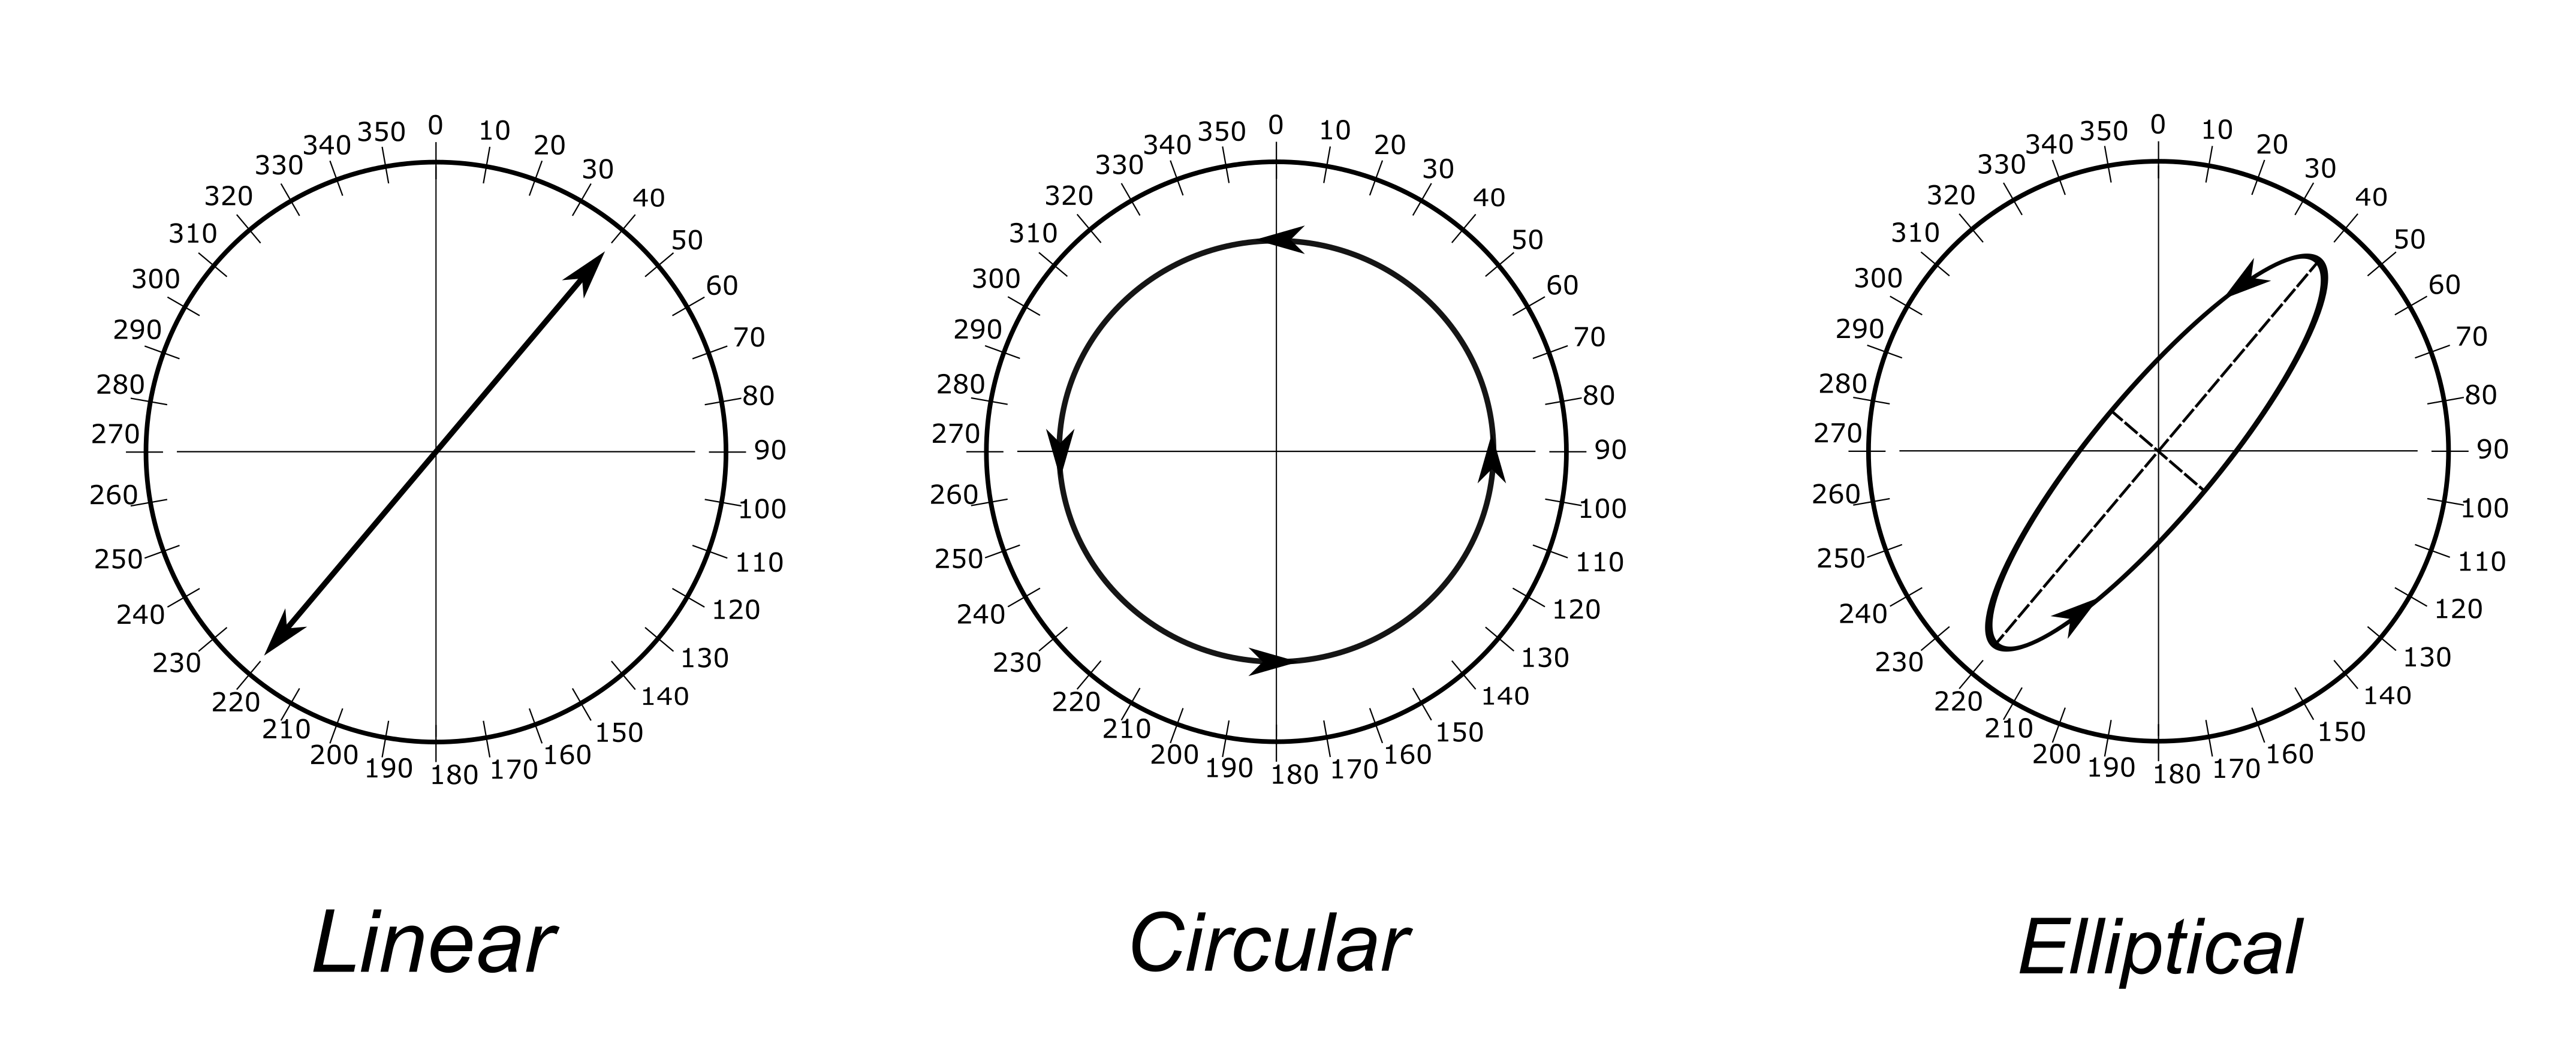
\includegraphics[width=5.37125in,height=2.215in]{images/11_polarization/linear-circular-elliptical.png}
  \caption*{\textbf{Types of polarization}. \emph{Here are shown the types of polarization of light discussed above. 
  The light is conceived to be traveling perpendicular to the plane of the page, and the arrows represent the directions
  of polarization. In this frame of reference, linearly polarized light that is oriented along the axis from 0$^{\circ}$ to 180$^{\circ}$ is said
  to be vertically polarized.}}
  \end{center}
\vspace*{-20pt}
\end{figure}

A simple piece of equipment we will use frequently is the linear polarizer. Instead of splitting beams of light into
two perpendicularly polarized components, linear polarizers allow light polarized along one axis to pass, 
and absorb all light polarized perpendicular to that axis. At intermediate angles, only some of the light passes.
As stated above, Malus specifies this relation. If $I_0$ is the intensity of the light that would pass if the axes of the polarizer and the entering light were aligned, and $\theta$ is the angle between them, then the intensity $I$ of the light 
that passes is
\begin{equation*}\tag{\text{Malus's Law}}
I = I_0 \cos^2 \theta.\footnote{Dirac formulates the law differently, as involving the sine, but only because he reckons the angle starting from 90$^{\circ}$ away. We will follow Malus's convention, as has become the norm.}
\end{equation*}
Many of the phenomena of polarization will prove crucial to our future study, so in this practicum we will verify Malus's Law experimentally, and begin to familiarize ourselves with some of the other equipment we'll be using in upcoming practica. 

That equipment includes a laser light source, a photodiode detector (with attached signal amplifier, power supply, and voltmeter), a depolarizer, a diffraction grating, several linear polarizers,  and two kinds of devices we have not yet discussed: half-wave plates, and quarter-wave plates.  The linear polarizers, half-wave plates, and quarter-wave plates all look nearly identical.  The half-wave plates are marked ''$\lambda /2$,'' and the quarter-wave plates are marked ''$\lambda /4$'' near their centers.  Descriptions of the effects of half- and quarter-wave plates are given in the relevant sections below and, for the curious, a longer account is offered in the final section of this chapter. Finally, the polarizers are set in disks with fine angle markings and all the elements are arranged together in a straight line on an optical bench, which will allow us to investigate the phenomena of polarization with exactitude, by measuring intensities of light at different angle settings of multiple polarizers. A schematic representation of the full setup is shown below and the positions are marked for later reference.

\begin{figure}[h] % Figure 5
  \begin{center}
    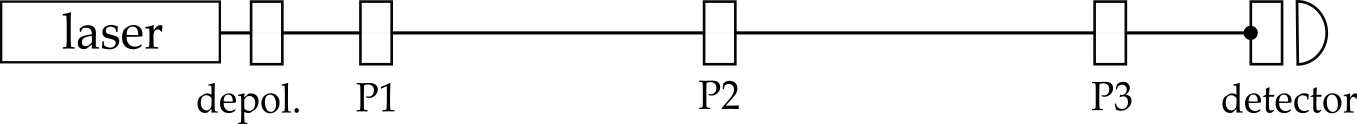
\includegraphics[width=4.5233in,height=0.4133in]{images/11_polarization/polarization-setup.png}
  \end{center}
\end{figure}

\section*{Practicum}

\begin{enumerate}[(A)]
	\item Begin by removing any optical elements that are attached to the bench standing between the laser and the detector. In order to remind ourselves of the wave-like properties of light, we can shine the laser light through a diffraction grating onto a piece of paper or an index card to reveal the characteristic interference pattern of dots that indicates maxima and minima of the light wave.

\item Next, we will examine the photodiode detector, used to measure the intensity of light passing through our various arrangements of polarizers. The sensitive element in the detector exploits the photoelectric effect. Here, unlike in the Einstein practicum, we are interested in only the magnitude of the overall current and not the kinetic energy of ejected electrons, since that current is proportional to the light intensity.
That said, the circuit we are using is designed (with the attached resistor) such that the electric potential generated by the device is proportional to current, and that voltage is more readily measured (with the help of the signal amplifier) than the current. All this by way of saying that the readings of light intensity will be in terms of DC voltage on the attached voltmeter. The power supply should be at 25V. Shine the the laser directly on the detector and read the voltage off the voltmeter. Obstruct the beam with your hand and watch the effect on the readings. Even moving your hand or body in the vicinity of the optics table can change the reading (slightly), so be aware of this in taking precise measurements.

\item The mechanics of the production of light are beyond us, especially in the case of light-emitting diodes or lasers. For us, a laser is simply a convenient light source, in two ways: it has a narrow beam that can be easily directed, and it is monochromatic, so that a color filter can screen out other sources of light, allowing us to make measurements with confidence. Because of the way it is produced, however, it happens that laser light is also typically linearly polarized, which we can confirm with a linear polarizer and the photodiode detector. Shine the laser light through a linear polarizer placed directly in front of the detector (at P3 in the diagram above). Determine the direction of polarization of the laser light by adjusting the angle of the linear polarizer to get the maximum signal from the detector.  The zero degree mark for the linear polarizer signifies vertical polarization plus or minus a few degrees.
Slowly rotate the polarizer to get the maximum and minimum readings and thereby determine the direction and degree of polarization of the laser light. The minima and maxima should be 90$^\circ$ apart.


\item As a consequence of the incomplete polarization of the laser light, just demonstrated, we will begin all our subsequent experiments on polarization by passing the light through a depolarizer. Set a linear polarizer in front of the detector at P3 and the smaller depolarizer in front of the laser (at the position marked ``depol.''). Confirm that the light is mostly depolarized by rotating the linear polarizer near P3 to different angles and noting the maximum and minimum voltage readings from the detector and their positions. Again, leave the depolarizer in place for all the measurements described below.


\item Interpose a second linear polarizer at P1 and align them as follows: Set the one closest to the detector at P3 to 0$^{\circ}$ and adjust the one at P1 to produce the maximum intensity reading, which should be near its 0$^{\circ}$, but may be as far as 15$^\circ$ away. Take care to note this deviation; this is the new ``zero'' for that polarizer and all your future readings must take it into account. Verify that when the polarizer at P1 is turned 90$^{\circ}$ from its aligned position no light passes (\emph{i.e.}, the voltmeter reads near zero) . A typical reading near zero here is 0.01V.

\item Now take measurements to verify Malus's law.  With the depolarizer in place, and linear polarizers at P1 and P3 and aligned for a maximum signal, take a baseline reading ($I_0$) and then adjust the angle ($\theta$) between the two polarizers (it shouldn't matter which you turn or which way you 
turn it) by 10$^{\circ}$ at a time until $\theta$ has passed through 90 degrees. Note the readings $I$ from the detector at each angle and compare them with the formula:
\begin{equation*}
I = I_0 \cos^{2} \theta.
\end{equation*}

\item Now, we will interpose a third linear polarizer at P2 between the first two (at P1 and P3). Before placing it there, align the polarizers at P1 and P3 for a maximum signal, with P3 set at 0$^\circ$ as a benchmark. Now place a third linear polarizer at P2 and adjust it until you get a maximum signal, your new $I_0$ for this experiment (likely slightly lower than without a polarizer at P2). Now turn the polarizer at P3 to 90$^{\circ}$. This 
should result in a near-complete extinction of the signal from the detector (around 0.01V). Next, set LP2 to 45$^{\circ}$ from its starting position and note the reading from the detector. Depending on your understanding of how the polarizers work, you might or might not be surprised. Try to acccount for your readings theoretically and quantitatively. On the basis of this account, make and test predictions about the results for other settings of the three polarizers. Is Malus's Law still in effect? What do linear polarizers \emph{do} to the light?

\item As noted above, we will make frequent use not only of linear polarizers but of so-called \emph{half-wave plates} as well. For practical purposes, it may be sufficient to simply describe their effect: they \emph{change} the direction of polarization of linearly polarized light by twice the difference in angle between their primary axis and that of the direction of polarization of the incoming light. We can demonstrate these effects by replacing the linear polarizer at P2 in the setup for (G) with a half-wave plate. Begin by aligning the linear polarizers at P1 and P3 in the usual way (for maximum signal with P3 at 0$^\circ$) and then put the half-wave plate between them at P2, and adjust it for a maximum reading on the detector (again, this should be near 0$^\circ$ and should be marked down as your new $I_0$ for any subsequent calculations). Turn P3 until the signal is at its minimum, which should be very nearly 90$^\circ$. Now turn the half-wave plate in the direction of increasing angle until the signal is at its maximum (which should be near 45$^\circ$). Note the reading on the detector. How does this differ from the analogous setup with three linear polarizers? Confirm the effect of the half-wave plate by setting it at, say, 15$^\circ$ and 30$^\circ$ away from the vertical and finding the corresponding angle settings for P3 that give the maximum signal.

\item A similar piece of equipment with a useful effect is the quarter-wave plate. Again, we begin with a description of the effect for which the device was created: vertically polarized light incident upon a quarter-wave plate aligned at 45$^\circ$ will emerge \emph{circularly} polarized. If you have time, try to produce and confirm this effect. Remove the half-wave plate from the setup for (H) and align the polarizers at P1 and P3 as usual. Place a quarter-wave plate at P2 and adjust it (near 0$^\circ$) to produce the maximum signal. You can adjust P3 to confirm that the light emerging from the quarter-wave plate is still vertically polarized. Turn P3 until the signal is at its minimum, near 90$^\circ$. Now turn the quarter-wave plate until the signal is at its maximum, which should be near 45$^\circ$. If the light emerging from the quarter-wave plate is circularly polarized, this should show up as an equality of intensities for all positions of the linear polarizer at P3. If it is unevenly distributed, you can try noting the maximum and minimum readings, adjusting the quarter-wave plate's orientation by a few degress, then measuring again to see whether your readings are closer to being consistent with circular polarization. If you still have time left, you can try to verify that the light passing through the quarter-wave plate in this way is circularly polarized and not just unpolarized, by interposing a second quarter-wave plate between P2 and P3 turned to 90$^\circ$; the second quarter-wave plate should emit linearly polarized light, which you will be able to confirm with the linear polarizer at P3.

\end{enumerate}

\section*{Additional Activities}

\begin{enumerate}[(J)]

\item The laboratory has samples of Iceland spar suitable for demonstrating the polarization of light without the intervention of lasers and other specially designed optical equipment. Draw a dot on a piece of paper, and place a sample of crystal on it. Rotate the crystal and note that while one image of the dot stays still (the ordinary ray), the other does not (the extraordinary ray). Place a second crystal atop the first so that all their faces are parallel. Note that in this orientation the image is not split a second time. Rotate the second crystal and note the appearance of two more dots, and their disappearance when the rotation reaches a right angle.

%% \item Beam splitter.

\end{enumerate}

%%%%%%%%%%%%%%

\section*{Waveplates}

Optical elements that affect the state of polarization of light as our half- and quarter-wave plates do are useful. They are made from materials like the calcite crystal in which polarization was first discovered. Materials like that are called \emph{birefringent} in that they refract incoming light in two different ways, depending on how its polarization aligns with their internal structure. A waveplate is a sample of this material suitably prepared so as to produce a definite effect such as the ones mentioned above.

Birefringent materials, because of their crystalline structure---that is, because of the regular arrangement of atoms within them---have different electrical properties and thus different refractive indices for components of light lying along their axes (again, \emph{cf}. Maxwell, \emph{Treatise on Electricity and Magnetism, vol. 2,} \S\S 794--797). This has the effect that light polarized along one of these axes moves slower (at least in terms of phase) than it does along the other. A half-wave plate is constructed so that light of a definite wavelength will have the component polarized along its ``slow'' axis retarded by one half a period. Perpendicularly related components of the light that emerges thus remain in phase with each other, such that the light is polarized linearly, just in a different direction. By contrast, the quarter-wave plate---which, as the name indicates, retards one component by a quarter-period---does not leave the components in phase with one another, with the result that linearly polarized light passing through it will not (if it is not aligned at 0$^\circ$ or 90$^\circ$) emerge linearly polarized, but will instead take on some kind of \emph{elliptical} polarization.

